
%%%%%%%%%%%%%%%%%%%%%%%%%%%%%%%%%%%%%%%%%%%%%%%%%%%%%%%%%%%%%%%%%%% 
%                                                                 %
%                           RESULTS                               %
%                                                                 %
%%%%%%%%%%%%%%%%%%%%%%%%%%%%%%%%%%%%%%%%%%%%%%%%%%%%%%%%%%%%%%%%%%% 
 
% \specialhead{INTRODUCTION}
\chapter{RESULTS}
\label{chapter:results}
In this chapter we discuss results of our simulation.  First in Section \ref{section:pd_constants_results}, we describe choosing of the constants for the proportional derivative controllers, which required proportional ($k_p$) and derivative ($k_d$) constants to control the rate at which changes were applied to the simulation, motivating the choice of values in Table \ref{tab:pd_constants}.  We then discuss choice of muscle strength constants, as well as the length and height of trial jumps in Section \ref{section:muscle_results}.  This section also gives an estimate for how strong a human leg with similar dimensions would be.  Section \ref{section:speed_frame_results} describes performance of the simulation as well as our method of collecting frame data.  Examples of this collected frame data is shown in Section \ref{section:image_results}.  Finally, we discuss limitations of our simulation and method in Section \ref{section:limitations}.

\section{Proportional Derivative Controller Constants}
\label{section:pd_constants_results}
The windup PD controller was given constants of $k_p = 0.25$ and $k_d = 0.25$.  These were chosen empirically to offset irregularities due to time step and slow convergence in the inverse kinematic solver.  With higher values, the translation of the pelvis results in the character's feet embedding in the ground plane due to too great a movement in a single frame.  The feet then fail to adjust as the inverse kinematic solver cannot converge quickly enough.  As opposed to a performance issue, this is a limitation of the inverse kinematics algorithm used, which was chosen due to simplicity so focus of this project could remain on the jump simulation.  

In most cases, the inverse kinematic solver converged within 30 iterations, but in this situation more than 300 iterations were required.  To compensate, we chose PD controller constants to adjust the rate of of change of the animation.  These values were found to generally produce smooth windup phases without compromising on speed of the animation too much, where speed refers to the amount of movement in each frame, which requires the frames to be played back at a different rate to achieve the desired rate of movement in the final animation.

The controller for re-balancing performed well with $k_p = k_d = 1$, with little noticeable change in results and only a change in rate of convergence for values at $k_p = k_d = 0.5$ and $k_p = k_d = 1.5$.  This showed that the main bottleneck for control in the model was the windup control, leading us to choose the value 1.

\section{Muscle Constants and Strength Intuition}
\label{section:muscle_results}
Muscle spring constants were tested in various configurations, with several trials run for each set of constants for varying distances, directions, and situations.  Animations were created for forward jumps between 1m and 2m for the normal human values and at 1m, 10m, and 100m for the super human, based on the analysis of the standing long jump by Wu et al\cite{longjump}.  A jump onto a box was also simulated, with 0.5m and 0.75m boxes for the normal human and 1m and 100m boxes for the super human, with normal human values chosen based on the work done by Arag\'{o}n-Vargas and Gross \cite{vertjump}.  The normal human muscle constants were additionally used for sideways jumping animations, as well as a more complex scene in which the character is made to jump from on top of a box, over an obstacle before finally landing on the ground.

%biomechanics of sport and exercise
Jump animations appear plausible, and the spring values result in forces similar to a human muscle.  Human muscles have about $30\frac{N}{cm^2}$ force per cross-sectional area\cite{biomech_sport}. We perform the following calculation as an intuitive estimation of the expected leg strength of the character. The character's leg thickness is about $0.20m$ forward to back narrowing towards the knee, with a left-right thickness of around $0.15m$. If we assume that skin is about $0.002m$ thick (2mm) and about $15\%$ of the remainder is subcutaneous fat, we are left with a $0.1683m$ by $0.1258m$ cross section.  This gives an axial cross sectional area of approximately $0.021m^2$.  We use a bone width of $0.05m$, giving a cross sectional bone area of $0.0025m^2$ which leaves an area of $0.019m^2$ of non-bone muscle.  If half of this is extensor muscle, then we have an approximate cross sectional area of $0.0095m^2$ or $95cm^2$.  This means that the estimated maximum isometric force for the muscle is $F = \left(30 \frac{N}{cm^2}\right) \left(95cm^2\right) = 2850N$.  With a $k$ of 20000, our muscle produces \[
	F = -k \left(\dfrac{r \sin (\pi - \theta)}{\sin \frac{\theta}{2}} \right)
\]
which for a joint bend of $\frac{\pi}{2}$ radians is $1414N$.  For comparison, a character with mass $80kg$ requires approximately $800N$ of force to counteract gravity's effects on their body, with additional force providing upward acceleration.  A force of $1500N$ would thus produce $700N$ excess, which would in turn accelerate the character at $\frac{m}{s^2}$.  The $k$ value was determined empirically, following the assumption that an average person has a max long jump in the range of 1.5m to 2m, estimated based on Wu et al \cite{longjump}.  A possible explanation is that our simulated character can perfectly execute the movement, maintaining balance and applying force, either handling or ignoring extraneous movements due to the simplifications and assumptions of our simulation.  This extra work that a real human must perform may contribute to this difference.
%  The character in our simulation has a femur length of 0.4m and a shin length of 0.33m.  Our muscle crossing the knee has anchor points set between the knee and the ankle, and the knee and hip.  These anchors are set at $0.2 * 0.33m = 0.066m$ and $0.9 * 0.4m = 0.36m$ respectively, where $0.2$ and $0.9$ are values in $[0,1]$ which indicate how far along the bone the anchor is set as described in \ref{subsection:skel_joints}.  This gives a total length for this muscle as $0.426m$ or $42.6cm$. 

The produced animations are plausible and recognizable as jump animations.  The character loads its limbs appropriately, giving the appearance of weight, and extends its knees, hips, and lastly ankles to show thrust corresponding to the usage of its muscles.  As in a real jump, the character extends its ankles last, the calf muscle providing the final thrust of the motion.


\section{Simulation Speed and Frame Collection}
\label{section:speed_frame_results}
The simulation runs in an interactive frame rate, with a delay on start up for the calculation of the sample field.  As long as the mass and the muscle constants remain the same, the sample field need not be re-calculated.  The sample field calculation is linear in the number of samples taken.  A major bottleneck aside from populating the sample field is the convergence of the inverse kinematic solver.  The solver is required to run every frame, usually for many iterations unless it has already converged.  While the cost is manageable due to the linear nature of the algorithm, the main issue is when convergence does not occur and the simulation must either stop and wait for the solver to catch up, or continue on and risk corrupting the simulation due to misplaced joints or limbs.  There are two major cases of this occurring: the character's feet sinking into the ground instead of the knees bending during windup and the character's feet prematurely breaking contact with the ground during thrust.  Our simulation suspends its activities when a compromising situation is detected, iterating the inverse kinematic solver until the issue is resolved.  The solver usually converges within a few frames, but this can add undesired time to the simulation and undesired frames to the animation.

Frame data was collected at a rate of 1 frame per 0.1s of simulation time, giving a frame rate of 10 frames per second.  This granularity was used to ensure capture of any irregularities in the simulation and to ensure changes in pose were recorded as shorter trials ran in under 1s of simulation time, though the real time was several seconds.  Finer granularity was found to have little benefit.  We show one of five frames in the tables discussed in section \ref{section:image_results} to reduce the size of the animation strips presented and thereby reduce the size of our tables.

\begin{table}[ht]
	\centering
	\scriptsize
	\begin{tabular}{| c | c | c | c | c | c | c |}
		\hline
		& Left Hip & Left Knee & Left Ankle & Right Hip & Right Knee & Right Ankle \\ \hline
		Global, Normal & 20000 & 20000 & 20000 & 20000 & 20000 & 20000 \\ \hline
		Varying, Normal & 20000 & 24000 & 16000 & 20000 & 24000 & 16000 \\ \hline
		Uneven Global, Normal & 16000 & 16000 & 16000 & 24000 & 24000 & 24000 \\ \hline
		Uneven Varying, Normal & 24000 & 28000 & 20000 & 16000 & 20000 & 12000 \\ \hline
		Global, Super & $1 \times 10^{10}$ & $1 \times 10^{10}$ & $1 \times 10^{10}$ & $1 \times 10^{10}$ & $1 \times 10^{10}$ & $1 \times 10^{10}$ \\ \hline
	\end{tabular}
	\caption[Table of spring constants for each trial]{This table shows muscle spring constants ($k$) values used for several trial runs.  Each column represents a muscle, described by the center joint which indicates the joint the muscle crosses and affects.  Each row represents a different trial, with a set of $k$ values.  Global runs used a uniform $k$ for one or both sides of the body, while varying runs used different spring constants for each muscle.  Uneven runs were meant to mimic a character with an injury or other source of imbalance where one leg was significantly stronger than the other.}
	\label{tab:run_k_vals}
\end{table}


%TODO should the frame data dump be moved to the appendix?
\section{Output Animations}
\label{section:image_results}

Several trials were run with different, empirically determined $k$ values as shown in Table \ref{tab:run_k_vals}.  The destination position was chosen for each to demonstrate the range of motions possible with our simulation.  Trials can be divided into several types: forward jumps, sideways jumps, and box jumps.  In a forward jump, the character starts from standing and jumps forward to a destination.  A sideways jump is the same, except requiring the character to jump to the right without first turning.  Box jumps required the character to jump from standing to land on an obstacle in front of them.  Additionally, a more complex scene was constructed, in which the character starts standing on a box.  The character then jumps off the box, over an obstacle, and lands on the floor below.  The complex scene is pictured in Figure \ref{fig:complex_scene}.  The box on which the character starts is 1m in height, and the obstacle is 1.4m in height.  To achieve the path shown, the destination was set at $(0, 1.5, 1)$, with the starting position at $(0, 0, 0)$.  Muscle spring constants were set for all muscles globally as $k=20000$.

Forward jumps are shown in Tables \ref{tab:forward_200k_g}, \ref{tab:forward_200k_v}, and \ref{tab:superman_forward}. For the super human, jump destinations were set 1m and 100m in front of the character's starting position.  For the normal human, jumps were set at 1m, 1.3m, 1.6m, and 1.9m, shown in Table \ref{tab:forward_200k_g} for a globally set k and in Table \ref{tab:forward_200k_v} for a varying k.  Box jumps are also included in these tables, with 1m, 10m, and 100m boxes for the super human and 0.5m and 1m for the normal human.  Animations were produced for normal human strength with both a globally set $k=20000$, where each muscle had the same constant, and varying with $k=20000\pm 4000$ as shown in Table \ref{tab:run_k_vals}.

In Table \ref{tab:forward_200k_u} we show forward jumping motions of 1.6m and 1.9m where the character has uneven strength in their legs.  These values were chosen similar to the normal human run.  There is little effect, which is why lengths shown were only at the extreme of distance possible for the character.  However, the character's right leg can be seen to dangle in the trial with varying $k$ values, indicating that more load is on the left leg.

To demonstrate the flexibility of a simulation-based animation, we also include a jump to the side.  The destination was specified as 1m, 1.3m, and 1.6m to the right, i.e. the direction $(1, 0, 0)$ relative to the character, of the character's start position.  Instead of the pelvis thrusting forward and up, in these trials the pelvis thrust is to the side and upwards as expected.  These animations are shown in Table \ref{tab:side_200k_g} and were collected with a global $k=20000$.

\newcommand{\floatedfig}[1]{\begin{subfigure}[h]{0.2\textwidth}\vspace{1mm}\includegraphics[width=\textwidth]{#1}\vspace{1mm}\end{subfigure}\hspace{0.025\textwidth}}
\newcommand{\framesubfig}[1]{\begin{subfigure}[h]{0.24\textwidth}\includegraphics[width=\textwidth]{#1}\end{subfigure}}

\begin{figure}[ht]
	\centering
	\begin{subfigure}[h]{\textwidth}
		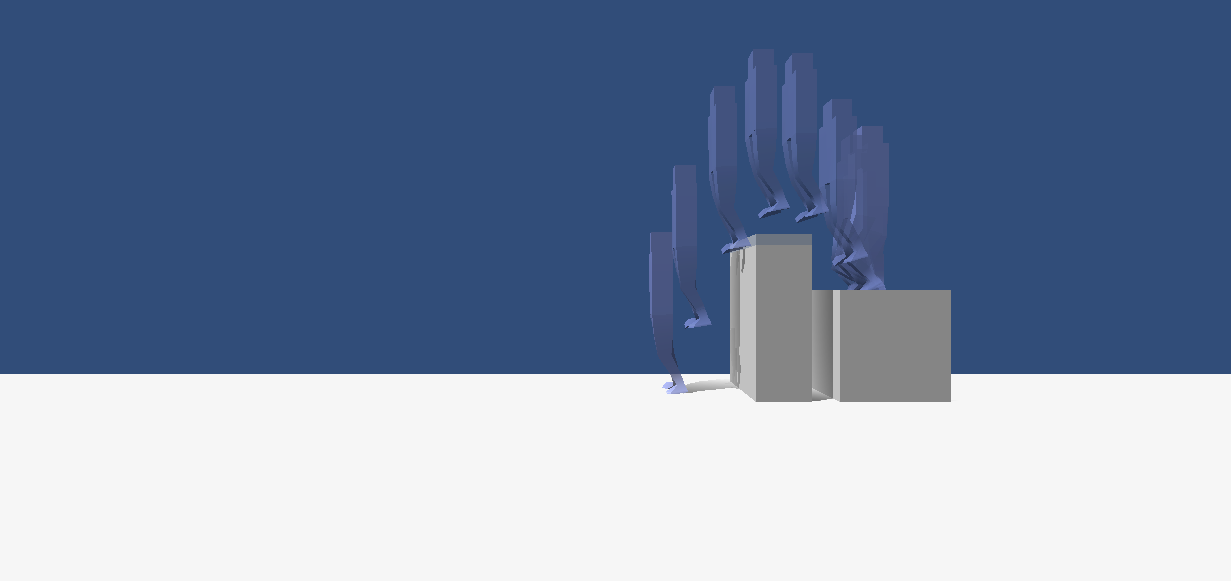
\includegraphics[width=\textwidth]{images/trials/K200000global/ComplexScene/BestPlacement/side-camera-composite.png}
	\end{subfigure}\vspace{1mm}
	%\raggedleft
	\framesubfig{images/trials/K200000global/ComplexScene/BestPlacement/side/frame0001.png}
	\framesubfig{images/trials/K200000global/ComplexScene/BestPlacement/side/frame0005.png}
	\framesubfig{images/trials/K200000global/ComplexScene/BestPlacement/side/frame0010.png}
	\framesubfig{images/trials/K200000global/ComplexScene/BestPlacement/side/frame0015.png}
	\framesubfig{images/trials/K200000global/ComplexScene/BestPlacement/side/frame0020.png}
	\framesubfig{images/trials/K200000global/ComplexScene/BestPlacement/side/frame0030.png}
	\framesubfig{images/trials/K200000global/ComplexScene/BestPlacement/side/frame0035.png}
	\framesubfig{images/trials/K200000global/ComplexScene/BestPlacement/side/frame0040.png}
	\framesubfig{images/trials/K200000global/ComplexScene/BestPlacement/side/frame0045.png}
	\framesubfig{images/trials/K200000global/ComplexScene/BestPlacement/side/frame0050.png}
	\framesubfig{images/trials/K200000global/ComplexScene/BestPlacement/side/frame0054.png}
	\caption[Animation of a jump over an obstacle]{Pictured is an animation of a complex scene, in which the character must jump from on top of a box, over another box and land on the ground.  The first image in the figure shows the frames composited into one image to visualize the full motion, while the remaining images show the individual frames.  This run used $t_{windup}=0.2s$ and $t_{air}=0.5s$.}
	\label{fig:complex_scene}
\end{figure}

\begin{table}[ht]
	\centering
	\begin{tabular}{|p{0.1\textwidth}|p{0.9\textwidth}|}
		\hline\vspace{1mm}
		1m forward &%
			\floatedfig{images/trials/K200000global/100cm/frame0001.png}
			\floatedfig{images/trials/K200000global/100cm/frame0005.png}
			\floatedfig{images/trials/K200000global/100cm/frame0010.png}
			\floatedfig{images/trials/K200000global/100cm/frame0015.png}
			\floatedfig{images/trials/K200000global/100cm/frame0020.png}
			\floatedfig{images/trials/K200000global/100cm/frame0024.png}
			\\ \hline
		1.3m forward &%
			\floatedfig{images/trials/K200000global/130cm/frame0001.png}
			\floatedfig{images/trials/K200000global/130cm/frame0005.png}
			\floatedfig{images/trials/K200000global/130cm/frame0010.png}
			\floatedfig{images/trials/K200000global/130cm/frame0015.png}
			\floatedfig{images/trials/K200000global/130cm/frame0020.png}
			\floatedfig{images/trials/K200000global/130cm/frame0024.png}
			\\ \hline
		1.6m forward &%
			\floatedfig{images/trials/K200000global/160cm/frame0001.png}
			\floatedfig{images/trials/K200000global/160cm/frame0005.png}
			\floatedfig{images/trials/K200000global/160cm/frame0010.png}
			\floatedfig{images/trials/K200000global/160cm/frame0015.png}
			\floatedfig{images/trials/K200000global/160cm/frame0020.png}
			\floatedfig{images/trials/K200000global/160cm/frame0024.png}
			\\ \hline
		1.9m forward &%
			\floatedfig{images/trials/K200000global/190cm/frame0001.png}
			\floatedfig{images/trials/K200000global/190cm/frame0005.png}
			\floatedfig{images/trials/K200000global/190cm/frame0010.png}
			\floatedfig{images/trials/K200000global/190cm/frame0015.png}
			\floatedfig{images/trials/K200000global/190cm/frame0020.png}
			\floatedfig{images/trials/K200000global/190cm/frame0025.png}
			\floatedfig{images/trials/K200000global/190cm/frame0028.png}
			\\ \hline
		0.5m box &%
			\floatedfig{images/trials/K200000global/50cmBox/frame0001.png}
			\floatedfig{images/trials/K200000global/50cmBox/frame0005.png}
			\floatedfig{images/trials/K200000global/50cmBox/frame0010.png}
			\floatedfig{images/trials/K200000global/50cmBox/frame0015.png}
			\floatedfig{images/trials/K200000global/50cmBox/frame0020.png}
			\floatedfig{images/trials/K200000global/50cmBox/frame0025.png}
			\floatedfig{images/trials/K200000global/50cmBox/frame0030.png}
			\floatedfig{images/trials/K200000global/50cmBox/frame0035.png}
			\floatedfig{images/trials/K200000global/50cmBox/frame0040.png}
			\floatedfig{images/trials/K200000global/50cmBox/frame0045.png}
			\\ \hline
		0.75m box &%
			\floatedfig{images/trials/K200000global/75cmBox/frame0001.png}
			\floatedfig{images/trials/K200000global/75cmBox/frame0005.png}
			\floatedfig{images/trials/K200000global/75cmBox/frame0010.png}
			\floatedfig{images/trials/K200000global/75cmBox/frame0015.png}
			\floatedfig{images/trials/K200000global/75cmBox/frame0020.png}
			\floatedfig{images/trials/K200000global/75cmBox/frame0025.png}
			\floatedfig{images/trials/K200000global/75cmBox/frame0030.png}
			\floatedfig{images/trials/K200000global/75cmBox/frame0035.png}
			\floatedfig{images/trials/K200000global/75cmBox/frame0039.png}
			\\ \hline
	\end{tabular}
	\caption[Table of frame sequences for forward and box jumps, $k=20000$ global]{Table of forward and box jump motions for a character with global $k=20000$, $t_{windup}=0.2s$, and $t_{air} = 0.5s$.  The boxes were placed 0.75m in front of the character, with the character's target destination set 0.3m in front of the character on top of the box.}
    \label{tab:forward_200k_g}
\end{table}

\begin{table}[ht]
	\centering
	\begin{tabular}{|p{0.1\textwidth}|p{0.9\textwidth}|}
		\hline\vspace{1mm}
		1m right &%
			\floatedfig{images/trials/K200000global/100cmRight/front/frame0001.png}
			\floatedfig{images/trials/K200000global/100cmRight/front/frame0005.png}
			\floatedfig{images/trials/K200000global/100cmRight/front/frame0010.png}
			\floatedfig{images/trials/K200000global/100cmRight/front/frame0015.png}
			\floatedfig{images/trials/K200000global/100cmRight/front/frame0020.png}
			\floatedfig{images/trials/K200000global/100cmRight/front/frame0025.png}
			\floatedfig{images/trials/K200000global/100cmRight/front/frame0030.png}
			\floatedfig{images/trials/K200000global/100cmRight/front/frame0035.png}
			\floatedfig{images/trials/K200000global/100cmRight/front/frame0040.png}
			\\ \hline
		1.3m right &%
			\floatedfig{images/trials/K200000global/130cmRight/front/frame0041.png}
			\floatedfig{images/trials/K200000global/130cmRight/front/frame0045.png}
			\floatedfig{images/trials/K200000global/130cmRight/front/frame0050.png}
			\floatedfig{images/trials/K200000global/130cmRight/front/frame0055.png}
			\floatedfig{images/trials/K200000global/130cmRight/front/frame0060.png}
			\floatedfig{images/trials/K200000global/130cmRight/front/frame0065.png}
			\floatedfig{images/trials/K200000global/130cmRight/front/frame0070.png}
			\floatedfig{images/trials/K200000global/130cmRight/front/frame0075.png}
			\floatedfig{images/trials/K200000global/130cmRight/front/frame0077.png}
			\\ \hline
		1.6m right &%
			\floatedfig{images/trials/K200000global/160cmRight/front/frame0078.png}
			\floatedfig{images/trials/K200000global/160cmRight/front/frame0083.png}
			\floatedfig{images/trials/K200000global/160cmRight/front/frame0088.png}
			\floatedfig{images/trials/K200000global/160cmRight/front/frame0093.png}
			\floatedfig{images/trials/K200000global/160cmRight/front/frame0098.png}
			\floatedfig{images/trials/K200000global/160cmRight/front/frame0103.png}
			\floatedfig{images/trials/K200000global/160cmRight/front/frame0108.png}
			\floatedfig{images/trials/K200000global/160cmRight/front/frame0111.png}
			\\ \hline
	\end{tabular}
	\caption[Table of frame sequences for sideways jumps, $k=20000$ global]{Table of right jump motions for a character with global $k=20000$, $t_{windup}=0.2s$, and $t_{air} = 0.5s$.  The target was placed at the distance listed in the table in the direction $(1, 0, 0)$ relative to the character.}
    \label{tab:side_200k_g}
\end{table}

\begin{table}[ht]
	\centering
	\begin{tabular}{|p{0.1\textwidth}|p{0.9\textwidth}|}
		\hline\vspace{1mm}
		1m forward &%
			\floatedfig{images/trials/K200000varying/100cm/frame0001.png}
			\floatedfig{images/trials/K200000varying/100cm/frame0005.png}
			\floatedfig{images/trials/K200000varying/100cm/frame0010.png}
			\floatedfig{images/trials/K200000varying/100cm/frame0015.png}
			\floatedfig{images/trials/K200000varying/100cm/frame0020.png}
			\floatedfig{images/trials/K200000varying/100cm/frame0024.png}
			\\ \hline
		1.3m forward &%
			\floatedfig{images/trials/K200000varying/130cm/frame0001.png}
			\floatedfig{images/trials/K200000varying/130cm/frame0005.png}
			\floatedfig{images/trials/K200000varying/130cm/frame0010.png}
			\floatedfig{images/trials/K200000varying/130cm/frame0015.png}
			\floatedfig{images/trials/K200000varying/130cm/frame0020.png}
			\floatedfig{images/trials/K200000varying/130cm/frame0024.png}
			\\ \hline
		1.6m forward &%
			\floatedfig{images/trials/K200000varying/160cm/frame0001.png}
			\floatedfig{images/trials/K200000varying/160cm/frame0005.png}
			\floatedfig{images/trials/K200000varying/160cm/frame0010.png}
			\floatedfig{images/trials/K200000varying/160cm/frame0015.png}
			\floatedfig{images/trials/K200000varying/160cm/frame0020.png}
			\floatedfig{images/trials/K200000varying/160cm/frame0024.png}
			\\ \hline
		1.9m forward &%
			\floatedfig{images/trials/K200000varying/190cm/frame0001.png}
			\floatedfig{images/trials/K200000varying/190cm/frame0005.png}
			\floatedfig{images/trials/K200000varying/190cm/frame0010.png}
			\floatedfig{images/trials/K200000varying/190cm/frame0015.png}
			\floatedfig{images/trials/K200000varying/190cm/frame0020.png}
			\floatedfig{images/trials/K200000varying/190cm/frame0025.png}
			\floatedfig{images/trials/K200000varying/190cm/frame0028.png}
			\\ \hline
		0.5m box &%
			\floatedfig{images/trials/K200000varying/50cmBox/frame0001.png}
			\floatedfig{images/trials/K200000varying/50cmBox/frame0005.png}
			\floatedfig{images/trials/K200000varying/50cmBox/frame0010.png}
			\floatedfig{images/trials/K200000varying/50cmBox/frame0015.png}
			\floatedfig{images/trials/K200000varying/50cmBox/frame0020.png}
			\floatedfig{images/trials/K200000varying/50cmBox/frame0030.png}
			\floatedfig{images/trials/K200000varying/50cmBox/frame0035.png}
			\floatedfig{images/trials/K200000varying/50cmBox/frame0040.png}
			\floatedfig{images/trials/K200000varying/50cmBox/frame0045.png}
			\floatedfig{images/trials/K200000varying/50cmBox/frame0046.png}
			\\ \hline
		0.75m box &%
			\floatedfig{images/trials/K200000varying/75cmBox/frame0001.png}
			\floatedfig{images/trials/K200000varying/75cmBox/frame0005.png}
			\floatedfig{images/trials/K200000varying/75cmBox/frame0010.png}
			\floatedfig{images/trials/K200000varying/75cmBox/frame0015.png}
			\floatedfig{images/trials/K200000varying/75cmBox/frame0025.png}
			\floatedfig{images/trials/K200000varying/75cmBox/frame0030.png}
			\floatedfig{images/trials/K200000varying/75cmBox/frame0035.png}
			\floatedfig{images/trials/K200000varying/75cmBox/frame0039.png}
			\\ \hline
	\end{tabular}
	\caption[Table of frame sequences for forward and box jumps, $k=20000$ varying]{Table of forward and box jump motions for a character with varying $k \approx 20000$, $t_{windup}=0.2s$, and $t_{air} = 0.5s$.  The boxes were placed 0.75m in front of the character, with the character's target destination set 0.3m in front of the character on top of the box.}
    \label{tab:forward_200k_v}
\end{table}

\begin{table}[ht]
	\centering
	\begin{tabular}{|p{0.1\textwidth}|p{0.9\textwidth}|}
		\hline\vspace{1mm}
		1.6m forward (global $k=20000$) &%
			\floatedfig{images/trials/K200000globaluneven/160cm/frame0001.png}
			\floatedfig{images/trials/K200000globaluneven/160cm/frame0005.png}
			\floatedfig{images/trials/K200000globaluneven/160cm/frame0010.png}
			\floatedfig{images/trials/K200000globaluneven/160cm/frame0015.png}
			\floatedfig{images/trials/K200000globaluneven/160cm/frame0020.png}
			\floatedfig{images/trials/K200000globaluneven/160cm/frame0025.png}
			\floatedfig{images/trials/K200000globaluneven/160cm/frame0030.png}
			\floatedfig{images/trials/K200000globaluneven/160cm/frame0035.png}
			\\ \hline
		1.9m forward (global $k=20000$) &%
			\floatedfig{images/trials/K200000globaluneven/190cm/frame0036.png}
			\floatedfig{images/trials/K200000globaluneven/190cm/frame0041.png}
			\floatedfig{images/trials/K200000globaluneven/190cm/frame0046.png}
			\floatedfig{images/trials/K200000globaluneven/190cm/frame0051.png}
			\floatedfig{images/trials/K200000globaluneven/190cm/frame0056.png}
			\floatedfig{images/trials/K200000globaluneven/190cm/frame0061.png}
			\floatedfig{images/trials/K200000globaluneven/190cm/frame0066.png}
			\\ \hline
		1.6m forward (varying $k=20000$) &%
			\floatedfig{images/trials/K200000varyinguneven/160cm/frame0001.png}
			\floatedfig{images/trials/K200000varyinguneven/160cm/frame0005.png}
			\floatedfig{images/trials/K200000varyinguneven/160cm/frame0010.png}
			\floatedfig{images/trials/K200000varyinguneven/160cm/frame0015.png}
			\floatedfig{images/trials/K200000varyinguneven/160cm/frame0020.png}
			\floatedfig{images/trials/K200000varyinguneven/160cm/frame0025.png}
			\floatedfig{images/trials/K200000varyinguneven/160cm/frame0030.png}
			\floatedfig{images/trials/K200000varyinguneven/160cm/frame0032.png}
			\\ \hline
		1.9m forward (varying $k=20000$) &%
			\floatedfig{images/trials/K200000varyinguneven/190cm/frame0001.png}
			\floatedfig{images/trials/K200000varyinguneven/190cm/frame0005.png}
			\floatedfig{images/trials/K200000varyinguneven/190cm/frame0010.png}
			\floatedfig{images/trials/K200000varyinguneven/190cm/frame0015.png}
			\floatedfig{images/trials/K200000varyinguneven/190cm/frame0020.png}
			\floatedfig{images/trials/K200000varyinguneven/190cm/frame0025.png}
			\floatedfig{images/trials/K200000varyinguneven/190cm/frame0030.png}
			\floatedfig{images/trials/K200000varyinguneven/190cm/frame0034.png}
			\\ \hline
	\end{tabular}
	\caption[Table of frame sequences for jumps with uneven leg strengths, $k=20000$ global]{Table of forward jumping motions with uneven muscle strengths between legs, using $t_{windup}=0.2s$ and $t_{air}=0.5s$.}
    \label{tab:forward_200k_u}
\end{table}

\begin{table}[ht]
	\label{tab:superman_forward}
	\centering
	\begin{tabular}{|p{0.1\textwidth}|p{0.9\textwidth}|}
		\hline
		1m forward &%
			\floatedfig{images/trials/k1e10global/1m/frame0001.png}
			\floatedfig{images/trials/k1e10global/1m/frame0005.png}
			\floatedfig{images/trials/k1e10global/1m/frame0011.png}
			\floatedfig{images/trials/k1e10global/1m/frame0015.png}
			\floatedfig{images/trials/k1e10global/1m/frame0020.png}
			\floatedfig{images/trials/k1e10global/1m/frame0025.png} 
			\floatedfig{images/trials/k1e10global/1m/frame0030.png}
			\floatedfig{images/trials/k1e10global/1m/frame0033.png}
			\floatedfig{images/trials/k1e10global/1m/frame0035.png}%
			\\ \hline%
		10m forward &%
			\floatedfig{images/trials/k1e10global/10m/1s1point5s/frame0042.png}
			\floatedfig{images/trials/k1e10global/10m/1s1point5s/frame0047.png}
			\floatedfig{images/trials/k1e10global/10m/1s1point5s/frame0050.png}
			\floatedfig{images/trials/k1e10global/10m/1s1point5s/frame0053.png}
			\floatedfig{images/trials/k1e10global/10m/1s1point5s/frame0055.png}
			\floatedfig{images/trials/k1e10global/10m/1s1point5s/frame0060.png}
			\floatedfig{images/trials/k1e10global/10m/1s1point5s/frame0064.png}
			\floatedfig{images/trials/k1e10global/10m/1s1point5s/frame0066.png}
			\floatedfig{images/trials/k1e10global/10m/1s1point5s/frame0070.png}
			\floatedfig{images/trials/k1e10global/10m/1s1point5s/frame0075.png}
			\floatedfig{images/trials/k1e10global/10m/1s1point5s/frame0080.png}
			\floatedfig{images/trials/k1e10global/10m/1s1point5s/frame0085.png}
			\floatedfig{images/trials/k1e10global/10m/1s1point5s/frame0090.png}
			\floatedfig{images/trials/k1e10global/10m/1s1point5s/frame0095.png}
			\floatedfig{images/trials/k1e10global/10m/1s1point5s/frame0101.png}
			\\ \hline%
	\end{tabular}
	\caption[Table of frame sequences for forward jumps, $k=1 \times 10^10$ global]{Above are generated frame sequences for the super human trial, where the $k$ values were chosen such that the character could leap over a tall building, a 100m tall box.  Animations above were generated for 1m, 10m, and 100m forward jumps.  The 100m forward jump is not pictured due to the difficulty of capture, as either the jump was out of the range of the camera or the camera was too far to clearly see the animation.}
\end{table}

\begin{table}[ht]
	\label{tab:superman_box}
	\centering
	\begin{tabular}{|p{0.1\textwidth}|p{0.9\textwidth}|}
		\hline\vspace{1mm}
		1m box &%
			\floatedfig{images/trials/k1e10global/1mBox/frame0001.png}
			\floatedfig{images/trials/k1e10global/1mBox/frame0005.png}
			\floatedfig{images/trials/k1e10global/1mBox/frame0010.png}
			\floatedfig{images/trials/k1e10global/1mBox/frame0020.png}
			\floatedfig{images/trials/k1e10global/1mBox/frame0025.png}
			\floatedfig{images/trials/k1e10global/1mBox/frame0030.png}
			\floatedfig{images/trials/k1e10global/1mBox/frame0035.png}
			\floatedfig{images/trials/k1e10global/1mBox/frame0039.png}
			\\ \hline%
		100m box &%
			\floatedfig{images/trials/k1e10global/100mBox/1s5s/frame0001.png}
			\floatedfig{images/trials/k1e10global/100mBox/1s5s/frame0005.png}
			\floatedfig{images/trials/k1e10global/100mBox/1s5s/frame0010.png}
			\floatedfig{images/trials/k1e10global/100mBox/1s5s/frame0015.png}
			\floatedfig{images/trials/k1e10global/100mBox/1s5s/frame0020.png}
			\floatedfig{images/trials/k1e10global/100mBox/1s5s/frame0025.png}
			\floatedfig{images/trials/k1e10global/100mBox/1s5s/frame0030.png}
			\floatedfig{images/trials/k1e10global/100mBox/1s5s/frame0035.png}
			\floatedfig{images/trials/k1e10global/100mBox/1s5s/frame0040.png}
			\floatedfig{images/trials/k1e10global/100mBox/1s5s/frame0045.png}
			\floatedfig{images/trials/k1e10global/100mBox/1s5s/frame0050.png}
			\floatedfig{images/trials/k1e10global/100mBox/1s5s/frame0055.png}
			\floatedfig{images/trials/k1e10global/100mBox/1s5s/frame0060.png}
			\floatedfig{images/trials/k1e10global/100mBox/1s5s/frame0065.png}
			\floatedfig{images/trials/k1e10global/100mBox/1s5s/frame0070.png}
			\floatedfig{images/trials/k1e10global/100mBox/1s5s/frame0075.png}
			\floatedfig{images/trials/k1e10global/100mBox/1s5s/frame0080.png}
			\floatedfig{images/trials/k1e10global/100mBox/1s5s/frame0085.png}
			\floatedfig{images/trials/k1e10global/100mBox/1s5s/frame0090.png}
			\floatedfig{images/trials/k1e10global/100mBox/1s5s/frame0095.png}
			\floatedfig{images/trials/k1e10global/100mBox/1s5s/frame0100.png}
			\floatedfig{images/trials/k1e10global/100mBox/1s5s/frame0105.png}
			\floatedfig{images/trials/k1e10global/100mBox/1s5s/frame0110.png}
			\floatedfig{images/trials/k1e10global/100mBox/1s5s/frame0115.png}
			\floatedfig{images/trials/k1e10global/100mBox/1s5s/frame0120.png}
			\floatedfig{images/trials/k1e10global/100mBox/1s5s/frame0125.png}
			\floatedfig{images/trials/k1e10global/100mBox/1s5s/frame0130.png}
			\floatedfig{images/trials/k1e10global/100mBox/1s5s/frame0135.png}
			\floatedfig{images/trials/k1e10global/100mBox/1s5s/frame0140.png}
			\floatedfig{images/trials/k1e10global/100mBox/1s5s/frame0145.png}
			\floatedfig{images/trials/k1e10global/100mBox/1s5s/frame0148.png}
			\\ \hline
	\end{tabular}
	\caption[Table of frame sequences for box jumps, $k=1 \times 10^10$ global]{Animations of 1m and 100m box jumps for the super human.  This run uses $t_{windup} = 1s$ and $t_{air} = 5s$.}
\end{table}

\section{Limitations}
\label{section:limitations}
Our system has a number of limitations and failure cases.  First is that there are many constants to be specified, which is work intensive but gives freedom to make wide changes to the animation by tuning parameters

There are numerous small issues with the calculations caused by strange or unexpected interactions.  Foremost is the behavior of rotations and angle measurement in \unity{}.  Angles are read and interacted with as Euler angles, pitch, roll, and yaw, or rotation about the x, z, and y axes respectively.  Rotations, however, are stored and calculated by the engine in the form of quaternions in order to avoid gimbal lock and allow smoother interpolation between rotations.  Due to the conversions between the two, and various manipulations that occur in the scene, this can result in angles not restricted to $[-360, 360]$ degrees, and can result in jumps between positive and negative angles.  A solution would be to restrict the angles to positive angles in the range $[0,360]$ for all calculations and manipulations, but this makes specifying constraints more complex.  

Problems with angle also arise as the angle of the joint does not necessarily reflect the angle between the bones.  For example, when the knee is fully extended, the joint angle stored in the object is 0, but the angle between the bones is $\pi$ radians.  A solution is to calculate the angle between the bones of the joint when needed using the dot product of the vectors between the joint and its parent and the joint and its child.  We did not realize that there was still an issue with angle specification as the issue was balanced out as the supplementary angle was used erroneously, but a fully correct implementation would be desirable for true consistency.  The data was collected with the flawed implementation, though as previously stated it produced similar results.

Movement of the upper body is very minimal, and is quite unlike a human performing a long jump.  This is likely due to the restriction of pelvis reposition to the region over the supporting polygon.  Humans frequently move their pelvises far behind their supporting polygon, compensating using the weight of their upper body.  The usage of rapid movement of the upper body to aid in acceleration is also a factor we do not consider, such as the effects of arm swing on a jump.

As our simulation was focused on the movements leading to the airborne phase, the handling of in air maneuvers and landing are overly simplistic.  After the character becomes airborne, the pelvis will generally be displaced in the direction of acceleration relative to the feet.  The character should maneuver while airborne such that their feet are in front of their body to prepare for landing.  For landing, a reverse of the windup for the energy simulation could be used, loading the muscles in the legs to offset the kinetic energy the character has from the jump, converting it to elastic energy in the muscles.  Landing and airborne phases should be handled ideally by a separate controller.

Our inverse kinematic solver is also very simple, and brings its own issues due to this simplicity.  This algorithm was chosen specifically to minimize time, effort, and resources spent on the inverse kinematic component, in favor of the simulation itself.  With a different inverse kinematic solver, better results could be achieved.

The output of our simulation is currently image frames as well as the direct visualization through \unity{}, as opposed to a key frame animation in a format such as FBX, which could be utilized in video games.  An \maya{}  plugin that runs our simulation would also be more useful for allowing creation of animations if a real-time frame rate cannot be achieved.

\section{Summary}
\label{section:results_summary}
Plausible animations were created, with empirically determined $k$ values around 20000.  Analysis shows different values would be theoretically more realistic, but the empirically determined values still produced reasonable animations.  Animations were produced for a normal strength human as well as a super human for forward standing jumps, sideways standing jumps, and box jumps.  A scene was constructed in which the character jumped from on top of a box, over an obstacle, and landed on the ground below to show a more complex scene.  We discussed in this chapter the values used and method for collecting data, and presented sets of frames collected from several simulations with a variety of scenes.  Animations depicted forward, sideways, and box jumps for a normal human range of strength and for a super human strength.  An animation of a character jumping over an obstacle was also presented.